\documentclass[normal,cyan]{elegantnote}
\usepackage{ctex}
\usepackage{amssymb}
\usepackage{array}
\usepackage{color}
\usepackage{cancel}
\usepackage{minted}
\usepackage{tikz}
\usepackage{algorithmic}
\usepackage{algorithm2e}
\usepackage{xeCJK}
\def\Z{{\mathbb Z}}
\def\R{{\mathbb R}}
\def\C{{\mathbb C}}
\def\Q{{\mathbb Q}}
\def\du{{^{\circ}}}
\newcommand{\limit}[2]{\lim\limits_{#1 \to #2}}
\newcommand{\Sum}[3]{\sum\limits_{#1 = #2}^{#3}}
\newcommand{\roma}[1]{\uppercase\expandafter{\romannumeral#1}}
\newtheorem{solve}{解}
\newcommand{\QED}{\square}
\newcommand{\stirling}[2]{\begin{Bmatrix}#1\\#2\end{Bmatrix}}
\newcommand*{\dif}{\mathop{}\!\mathrm{d}}
\usetikzlibrary{arrows, graphs}

\title{Note for Discrete Mathematics}
\date{\today}
\institute{\href{http://leadedglass.site}{my blog}}

\begin{document}

\maketitle
\tableofcontents
\newpage

\section{第 \roma{1} 章}
\subsection{数理逻辑}

1. 数理逻辑属于形式逻辑,是在形式上符号化、数学化的逻辑。数理逻辑又称符号逻辑、理论逻辑。它既是数学的一个分支,也是逻辑学的一个分支。是用数学方法研究逻辑或形式逻辑的学科。

2. \textbf{数理逻辑} = 命题逻辑 + 谓词逻辑。

\subsubsection{命题逻辑}
1. 命题是一个能判断真假的陈述句。

\begin{note}
    在离散数学中,”宇宙中存在外星人“为 $\textbf{T}$。
\end{note}

2. 不能用\textbf{更简单}的命题来表示的命题称为\textbf{原子命题}。

3. 三个常见的逻辑联结词:否定($\neg$),析取($\vee$),合取($\wedge$)。
\\
    析取与异或一个常见的区别是,析取又被称为“包容性或”,若 $p \vee q$ 为真,那么只需其中一个为真即可;
而异或又被称为“排他性或”,若 $p \bigoplus q$ 为真,那么其中一个必须为真,但两个不能同时为真。
\\
    如下为否定、析取、合取、异或的真值表:

\begin{table}[htbp]\centering
    \begin{tabular}{|l|l|l|l|l|l|}
    \hline
    p & q & $\neg$ p & p $\vee$ q & p $\wedge$ q & p $\bigoplus$ q \\ \hline
    T & T & F             & T          & T            & F               \\ \hline
    T & F & F             & T          & F            & T               \\ \hline
    F & T & T             & T          & F            & T               \\ \hline
    F & F & T             & F          & F            & F               \\ \hline
    \end{tabular}
    \end{table}
否定可以写作 $\neg p$ 或 $\overline{p}$,但也有更多的写法,如:$\sim p,p',\mathrm{N}p,!p$。

4. 蕴含式:令 $p$ 和 $q$ 为命题,条件语句 $p\to q$ 是命题“若 $p$ ,则 $q$”,\textbf{当 $p$ 为真而 $q$ 为假时,$p\to q$ 为假,否则为真}。$p$ 称为假设(前件,前提),$q$ 称为结论(后件)。条件语句也称为\textbf{蕴含}。

\begin{note}
    $p \to q \equiv \neg p \vee q$。
    \\在 $p \to q$ 中,前因和后果之间不需要任何联系,$p \to q$ 的值只取决于 $p$ 和 $q$ 的真值,不取决于其他命题的真值。\\ 前提或前提为假,则 $p \to q$ 必为真。(啊对对对了属于是
\end{note}

5. $p \to q$ 的逆命题为 $q \to p$,否命题为 $\neg p \to \neg q$,逆否命题为 $\neg q \to \neg p$。原命题与逆否命题具有相同的真值。

6. 命题 $p\leftrightarrow q$ 读作“$p$ 当且仅当 $q$”,称为双条件语句,也被称为\textbf{双向蕴含}。真值表如下:
\begin{table}[htbp]\centering
    \begin{tabular}{|l|l|l|}
    \hline
    p & q & $p \leftrightarrow q$ \\ \hline
    T & T & T                     \\ \hline
    T & F & F                     \\ \hline
    F & T & F                     \\ \hline
    F & F & T                     \\ \hline
    \end{tabular}
    \end{table}

\begin{note}
    其他几种表达“$p$ 当且仅当 $q$”的方式:1. $p$ 是 $q$ 的充分必要条件;2. 如果 $p$,则 $q$,反之亦然;3. $p$ $\text{iff}$ $q$。
    \\ $p \leftrightarrow q\equiv \neg\left(p \bigoplus q\right) \equiv \left(p \to q\right) \wedge \left(q \to p \right)$。
\end{note}

7. 逻辑命题的优先级:$\neg,\ \wedge,\ \vee,\ \to,\ \leftrightarrow$。

\begin{theorem}$n$ 个命题变元,不等价的公式有 $2^{2^n}$ 个,有 $2^n$ 行。\end{theorem}
\begin{proof}
    由于每个命题变元都只有两种可能的值,于是,由乘法原理知 $n$ 个命题变元可能值的组合为 $2^n$。
    
    对于不等价的公式,只要对于每一行所取的真值均不同即可,于是对于任意一行均有 $2$ 个不同的公式,对于 $2^n$ 行则有 $2^{2^n}$ 个不同的公式。$\QED$
\end{proof}

8. 将语句转换成命题逻辑语句的步骤:
\begin{enumerate}[a)]
    \item 找出原子命题并用命题变量表示;
    \item 给定合适的逻辑联结词。
\end{enumerate}

\begin{example}
    将下列句子翻译成命题逻辑:“只有你是计算机科学专业的学生或者不是大一新生,你才能从学校上网。”
\end{example}
\begin{solve}一种解:令 $a$,$c$,$f$ 分别为“你可以从校园上网”、“你是计算机科学专业的学生”和“你是大一新生”,那么可以得到 $a \to \left(c \vee \neg f\right)$。\end{solve}
\begin{remark}
    注意,$c \vee \neg f$ 不可写成 $c \leftrightarrow \neg f$,由于能在校园上网的人不一定只有学生,比如老师也可以从学校上网,但他不是大一新生。
\end{remark}

9. 系统规范一致:一个命题含有多个命题变元。如果能够给命题变量赋真值,使每个命题为真,那么这些命题是一致的。
\begin{example}
    以下规范是否一致?\\
“诊断消息存储在缓冲区中或重传。”\\
“诊断消息没有存储在缓冲区中。”\\
“如果诊断消息存储在缓冲区中,则重传。”
\end{example}
\begin{solve}令 $p$ 表示“诊断消息存储在缓冲区中”,$q$ 表示“诊断消息重传”,则规范可以写为 $p \vee q$,$p \to q$,$\neg p$。
当 $p$ 为假且 $q$ 为真时,三个陈述都为真,因此规范一致。\end{solve}
\begin{note}
    如果加上“没有重新传输诊断消息”,则规范中加入一个 $\neg q$,可以发现此时没有满足要求的组合,因此规范不一致。
\end{note}

10. 重言式、矛盾式和可能式:一个真值永远是真的命题,称为\textbf{永真式},也称为重言式;一个真值永远是假的命题,称为\textbf{矛盾式};既不是永真式也不是矛盾式的命题称为\textbf{可能式}。

11. 如果 $p\leftrightarrow q$ 是永真式,则称 $p$ 和 $q$ 是\textbf{逻辑等价}的,记作 $p\Longleftrightarrow q$ 或 $p\equiv q$ 。
当且仅当真值表中给出真值的列一致时,两个复合命题p 和q 是等价的。

12. De Morgan 定律:$\neg\left(p\wedge q\right)\equiv \neg p \vee \neg q$, $\neg\left(p \vee q\right) \equiv \neg p \wedge \neg q$。

13. 常用的逻辑等价式:
\begin{enumerate}[1)]
    \item 恒等律:$p\wedge \mathbf{T} = p,p\vee \mathbf{F} = p$
    \item 支配律:$p \wedge \mathbf{F} = \mathbf{F},p \vee \mathbf{T} = \mathbf{T}$
    \item 幂等律:$p \wedge p = p,p \vee p = p$
    \item 双非律:$\neg(\neg p) = p$
    \item 否定律:$p \vee \neg p = \mathbf{T},p \wedge \neg p = \mathbf{F}$
    \item 交换律:$p\wedge q = q \wedge p, p \vee q = q \vee p$
    \item 结合律:$(p\wedge q)\wedge r = p \wedge (q \wedge r),(p\vee q) \vee r=p\vee(q\vee r)$
    \item 分配律:$p\vee(q\wedge r) = (p\vee q)\wedge(p\vee r),p\wedge(q\vee r) = (p\wedge q)\vee(p\wedge r)$
    \item 吸收律:$p\vee(p\wedge q) = p,p\wedge(p\vee q) = p$
\end{enumerate}

14. 其他的逻辑等价式:
\begin{enumerate}[1)]
    \item $p \to q \equiv \neg p \vee q$
    \item $p \to q \equiv \neg q \to \neg p$
    \item $p \vee q \equiv \neg p \to q$
    \item $p \wedge q \equiv \neg\left(p \to \neg q\right)$
    \item $\neg \left(p \to q\right) \equiv p \wedge \neg q$
    \item $(p \rightarrow q) \wedge(p \rightarrow r) \equiv p \rightarrow(q \wedge r)$
    \item $(p \rightarrow r) \wedge(q \rightarrow r) \equiv(p \vee q) \rightarrow r$
    \item $(p \rightarrow q) \vee(p \rightarrow r) \equiv p \rightarrow(q \vee r)$
    \item $(p \rightarrow r) \vee(q \rightarrow r) \equiv(p \wedge q) \rightarrow r$
    \item $p \leftrightarrow q \equiv(p \rightarrow q) \wedge(q \rightarrow p)$
    \item $p \leftrightarrow q \equiv \neg p \leftrightarrow \neg q$
    \item $p \leftrightarrow q \equiv(p \wedge q) \vee(\neg p \wedge \neg q)$
    \item $\neg(p \leftrightarrow q) \equiv p \leftrightarrow \neg q$
\end{enumerate}

15. 析取范式:如果命题公式由 $(1,\dots,n)$ 个析取组成,则它是\textbf{析取范式},其中\text{每个析取}由 $(1,\dots,m)$ 个\textbf{原子公式的合取或否定组成}。如 $(p\wedge\neg q)\vee(\neg p\wedge q)$ 。
\\ \textbf{每个}复合命题公式都可以等价地转换成一个析取范式。
\\ 主析取范式:每个小项中均包含所有命题变量。
\begin{note}
    主析取范式一定是析取范式,但析取范式不一定是主析取范式。
    \\永假式不存在析取范式。
    \\求一个复合命题的析取范式的步骤:
    \begin{enumerate}[1)]
        \item 做出复合命题的真值表;
        \item 找出值为 $\mathbf{T}$ 的行;
        \item 列出每行对应的小项,求这些小项的析取式。
    \end{enumerate}
\end{note}
\begin{example}
    求 $A = \left(p \wedge q \right) \vee \left(\neg p \wedge r\right) \vee \left(q \wedge r\right)$ 的主析取范式。
\end{example}
\begin{solve}
    $A \Longleftrightarrow (p \wedge q \wedge(r \vee \neg r)) \vee (\neg p \wedge r \wedge(q \vee \neg q)) \vee (q \wedge r \wedge(p \vee \neg p))\\
        \Longleftrightarrow (p \wedge q \wedge r) \vee (p \wedge q \wedge \neg r) \vee (\neg p \wedge r \wedge q) \vee (\neg p \wedge r \wedge \neg q).
    $
\end{solve}
\begin{remark}
    用等价变换法求主析取范式的步骤:
    \begin{enumerate}[1)]
        \item 化归为析取范式;
        \item 除去析取范式中所有永假的析取项;
        \item 将析取项中重复出现的合取项和相同的变元合并;
        \item 对合取项补入没有出现的命题变元(如 $p \vee \neg p$),然后应用分配律展开公式。
    \end{enumerate}
\end{remark}
16. 合取范式:如果命题公式由 $(1,\dots,n)$ 个合取组成,则它是\textbf{合取范式},其中\text{每个合取}由 $(1,\dots,m)$ 个\textbf{原子公式的析取或否定组成}。
\\ 类似地,每个复合命题公式也可以等价地转换成一个合取范式。
\\ 主合取范式:每个大项均包含所有命题变量。
\\ 永真式不存在合取范式。
\begin{example}
    将 $\neg(p \to q) \to (r \to p)$ 转换为合取范式。
\end{example}
\begin{solve}
    \begin{enumerate}[1)]
        \item 首先消除蕴含式:$\neg(\neg p \vee q) \vee (\neg r \vee p)$
        \item 向括号内移动否定式消除双重否定:$(p \wedge \neg q) \vee (\neg r \vee p)$
        \item 使用结合律或分配律转换为合取范式:$(p \vee \neg r \vee p) \wedge (\neg q \vee \neg r \vee p)$
        \item 化简整个等价公式得到结果。
    \end{enumerate}
\end{solve}
命题公式转化为其主合取范式的步骤:
\begin{enumerate}[1)]
    \item 化归为合取范式;
    \item 除去合取范式中所有为永真的合取项;
    \item 合并相同的析取项和相同的变元;
    \item 对析取项补入没有出现的命题变元(如 $p \wedge \neg p$),然后应用分配律展开公式。
\end{enumerate}
\begin{example}
    将 $(p \wedge q) \vee (\neg p \wedge r)$ 化简为主合取范式。
\end{example}
\begin{solve}
    $(p \wedge q) \vee (\neg p \wedge r) \Longleftrightarrow ((p \wedge q) \vee \neg p) \wedge ((p \wedge q) \vee r) \\
    \Longleftrightarrow (p \vee \neg p) \wedge (q \vee \neg p) \wedge (p \vee r) \wedge (q \vee r) \\ 
    \Longleftrightarrow (q \vee \neg p) \wedge (p \vee r) \wedge (q \vee r) \\
    \Longleftrightarrow (q \vee \neg p \vee (r \wedge \neg r))\wedge (p \vee r \vee (q \wedge \neg q)) \wedge (q \vee r \vee (p \wedge \neg p)) \\
    \Longleftrightarrow (q \vee \neg p \vee r) \wedge (q \vee \neg p \vee \neg r) \wedge (p \vee r \vee q) \wedge (p \vee r \vee \neg q) \wedge (q \vee r \vee p) \wedge (q \vee r \vee \neg p) \\
    \Longleftrightarrow (\neg p \vee q \vee r) \wedge (\neg p \vee q \vee \neg r) \wedge (p \vee \neg q \vee r) \wedge (p \vee q \vee r).
    $
\end{solve}
\begin{note}
    小项即为 $n$ 个布尔变元的合取式,大项即为 $n$ 个布尔变元的析取式。

    在任一小项或大项中,每个变元和它的否定必须出现且仅出现一次。
\end{note}
17. 命题可满足性:如果在各种真值指派下至少存在一组成真指派,那么这个复合命题是可以满足的。当没有这样的指派存在时,复合命题是不能满足的。

当且仅当复合命题的否定是重言式时,复合命题是不可满足的。
\begin{example}
    确定 $(p \vee \neg q) \wedge (q \vee \neg r) \wedge (r \vee \neg p)$ 的可满足性。
\end{example}
\begin{solve}
    当 $p$,$q$,$r$ 的值均为$\mathbf{T}$ 时,命题为真,于是该命题可满足。
\end{solve}
\begin{example}
    确定 $(p \vee \neg q) \wedge (q \vee \neg r) \wedge (r \vee \neg p) \wedge (p \vee q \vee r) \wedge (\neg p \vee \neg q \vee \neg r)$ 的可满足性。
\end{example}
\begin{solve}
    它是不可满足的,当尝试命题变量的每一种可能的真值赋值,没有一个会使命题为真。
\end{solve}
18. 设 $p$ 和 $q$ 为两个命题,复合命题 $p \uparrow q$ 称为 $p$ 和 $q$ 的“与非”, $p \downarrow q$ 称为 $p$ 和 $q$ 的“或非”。

19. 最小联结词组:能表示所有命题的含有最少联结词的联结词组,如 $\{\neg, \vee\}$,$\{\neg , \wedge\}$,$\{\uparrow\}$,$\{\downarrow\}$。
\begin{proof}
    设最小联结词组中联结词的个数为 $n$。考虑 $n = 1$ 时,如果只有 $\vee$ 或 $\wedge$ 则无法表示否定命题,因此不可能表示所有命题,对于只有 $\neg$ 的情况类似。

    当 $n = 2$ 时,由于任意一个命题公式都可以等价地转换为一个析取范式或合取范式,于是 $\{\neg, \vee\}$ 或 $\{\neg , \wedge\}$ 均可以表示所有命题。$\QED$
\end{proof}
20. 对偶原理:对于一个逻辑等值式,如果 \textbf{只含有} $\wedge, \vee, \neg, 0, 1$,那么\textbf{同时} 把 $\wedge$ 和 $\vee$ 互换,$0$ 和 $1$ 互换,得到的还是一个等值式。

21. $A \Longrightarrow B$ 当且仅当 $A\rightarrow B$ 是永真式,读作 $A$ 推出 $B$ 。

22. 设 $X$ 是合式公式 $A$ 中的一个部分,且 $X$ 也是一个合式公式,则称 $X$ 是 $A$ 的一个\textbf{子公式}。
\begin{theorem}[置换规则]
    设 $X$ 是合式公式 $A$ 中的子公式,若 $Y$ 是一个合式公式,且 $X \Longleftrightarrow Y$,用 $Y$ 置换 $A$ 中的 $X$,得到新的合式公式 $B$,则 $A \Longleftrightarrow B$。
\end{theorem}
\begin{proof}
    $A$ 与 $B$ 除替换部分外均相同,又由于替换部分 $X \Longleftrightarrow Y$,即是说对任一指派,$X$ 和 $Y$ 真值相同,那么 $A$ 对 $B$ 对任一真值指派也应有相同的真值,于是 $A \Longleftrightarrow B$。$\QED$
\end{proof}
23. 给定命题公式 $A(P_1, P_2, \dots, P_n)$,如果用某个命题公式 $B_i$ 取代 $A$ 中的某个变元 $P_i$,并且用 $B_i$ 取代 $A$ 中所有出现的所有 $P_i$,这样得到的命题公式 $B$ 称为命题公式 $A$ 的一个\textbf{代入实例}。
\begin{theorem}[代入规则]
    一个重言式的代入实例仍然是一个重言式。
\end{theorem}
\begin{proof}
    由于重言式的真值与真值指派无关,故对同一命题变元都用某个命题公式代替,该重言式的真值仍为 $\mathbf{T}$。$\QED$
\end{proof}
\begin{example}
    证明 $((p \vee s) \wedge r) \vee \neg((p \vee s) \wedge r)$ 为重言式。
\end{example}
\begin{solve}
    由于 $p \vee \neg p \Longleftrightarrow \mathbf{T}$,于是根据代入规则可以得到原式为重言式。
\end{solve}
\begin{example}
    有一个含 $100$ 条语句的列表,其中第 $n$ 条语句写的是“列表中恰有 $n$ 条语句为假”。
    \begin{enumerate}[a)]
        \item 你能从这些语句中得出什么结论?
        \item 如果第 $n$ 条语句写的是“列表中至少有 $n$ 句语句为假”,回答问题 a。
        \item 假设这个列表包含 $n$ 条语句,回答问题 b。
    \end{enumerate}
\end{example}
\begin{solve}
    \begin{enumerate}[a)]
        \item 容易发现,只有第 $99$ 条语句是真的,这样才能保证不出现逻辑矛盾。
        \item 由于是“至少有 $n$ 条语句为假”,那么前一半可以全部成立,即在前一半语句成立时都不会出现逻辑矛盾,而当多于一半的语句成立时,为假的语句将会少于一半,这样就会出现逻辑矛盾。
        \item 如 $\text{b)}$ 所示,对于 $n$ 为偶数的情况,前一半命题均可以成立,后一半命题均不可能成立。奇数情况通过类似的考虑发现,$1 \sim \lfloor \frac {n}{2} \rfloor $ 均可以成立,$\lceil  \frac {n}{2} \rceil  + 1  \sim n$ 均不能成立,考虑第 $\lceil  \frac {n}{2} \rceil$ 条,如果第 $\lceil  \frac {n}{2} \rceil$ 条为真,那么此语句所叙述的事实应当为假,反之亦然。于是这是一个悖论,不可能出现如此的列表。
    \end{enumerate}
\end{solve}
\subsubsection{谓词逻辑}
1. 一般地,涉及 $n$ 个变量 $x_1, x_2, \dots, x_n$ 的语句可以表示为 $\displaystyle P(x_1, x_2, \dots, x_n)$ 形式为 $$P(x_1, x_2, \dots, x_n)$$ 的语句是\textbf{命题函数} $P$ 在 $n$ 元组 $(x_1, x_2, \dots, x_n)$ 的值。$P$ 也称为\textbf{$n$ 位谓词}或\textbf{$n$ 元谓词}。
\begin{remark}
    谓词把原子命题分成了两部分,分别描述,所以谓词逻辑是更加精细化的命题逻辑。

    比如三个命题:张三能爬上那座山。汽车能爬上那座山。老虎能爬上那座山。用谓词逻辑可以表示为:$X$ 能爬上那座山,个体域 $X = \{\text{张三,汽车,老虎}\}$。
\end{remark}
2. 两个重要的量词:全称量词 $\forall$,存在量词 $\exists$,分别写作 $\forall xP(x)$ 和 $\exists xP(x)$。
\begin{note}
    有一个唯一性量词 $\exists ! xP(x)$,它与 $\exists x(P(x) \wedge \forall y(P(y) \to y = x))$ 等价。

    许多命题对于变量在某一特定域内的所有值都为真,这一特定域称为变量的\emph{论域}(或\emph{全体域}),时常称之为\emph{域}。
    使用全称量词时必须指定论域,否则语句的\textbf{全称量化}就是无意义的。
\end{note}
3. $\exists xP(x)$ 和 $\forall xP(x)$ 的真值取决于命题函数 $P(x)$ 和论域 $U$。

4. 量词 $\forall$ 和 $\exists$ 的优先级高于其他所有逻辑运算符。
\begin{example}
    $\forall xP(x)\vee Q(x)$ 与 $(\forall xP(x)) \vee Q(x)$ 等价,而不与 $\forall x(P(x) \vee Q(x))$ 等价。
\end{example}
下面放个非常 sb 的例题(我知道很 sb 但还是放进来的原因是怕自己 sb 了把这个弄错
\begin{example}
    将以下句子翻译成谓词逻辑:“本班级中的每个学生都进修过 Java 课程。”
\end{example}
\begin{solve}
    如果 $U$ 是班级中的所有学生,则定义一个函数 $J(x)$ 表示“$x$ 已经学习了 Java 课程”,则命题为 $\forall xJ(x)$;

    如果 $U$ 是所有人,还需要定义一个函数 $S(x)$ 表示 “$x$ 是这个班级中的学生”,则命题为 $\forall x(S(x) \to J(x))$。

    需要注意到,$\forall x(S(x) \wedge J(x))$ 是错误的,这表示所有人都是这个班级里的学生,显然不成立。
\end{solve}
5. 如果论域是有限的,那么全称量词的命题等价于合取的命题,存在量词的命题等价于析取的命题。即使论域是无限的,仍然可以用上面这种方式理解量词,但没有量词的等价表达式是无限长的。

如果 $U = \{1, 2, 3\}$,则 $\forall xP(x) = P(1)\wedge P(2) \wedge P(3)$,$\exists xP(x) = P(1) \vee P(2) \vee P(3)$。

6. 量词的 De Morgan 定律:$\neg \forall xP(x) \equiv \exists x\neg P(x)$,$\neg \exists xP(x) \equiv \forall x\neg P(x)$。

7. 关于嵌套量词:
\begin{example}
    $\forall x \exists yP(x, y) \equiv \exists y \forall xP(x, y)$ 和 $\forall (P(x) \to Q(x)) \equiv \forall xP(x) \to \forall xQ(x)$ 是有效的等价吗?
\end{example}
\begin{solve}
    对于第一个等价,可以举出一个反例 $x + y = 0$,$\forall x \exists y$ 必然成立,而 $\exists y \forall x$ 不能成立,例如 $y = 1$ 时只有 $x = -1$ 才能满足 $x + y = 0$;\\
    第二个等价也是不正确的,设 $P(x)$ 为“$x$ 是鱼”,$Q(x)$ 为“ $x$ 有鱼鳞”,论域为所有动物,显然不等价。
\end{solve}
8. 合式公式中的变项:
\begin{enumerate}[1)]
    \item 量词辖域:在 $\exists xA$,$\forall xA$ 中,$A$ 是量词的辖域。
    \item 指导变项:紧跟在量词后面的个体变项。如:$\exists {\color{red} x}(F(x) \wedge \forall {\color{blue} y}(G(y) \to H(x, y)))$。
    \item 约束出现:在辖域中与指导变项同名的变项。如:$\exists x(F({\color{red} x}) \wedge \forall y(G({\color{blue} y}) \to H({\color{red} x}, {\color{blue} y})))$。
    \item 自由出现:既非指导变项又非约束出现的变项。如:$\forall y(G(y) \to H({\color{red} x}, y))$。
\end{enumerate}
\begin{theorem}[换名规则]
    把某个\textbf{指导变项}和其量词辖域中所有同名的\textbf{约束出现}, 都换成某个新的个体变项符号后得到的公式与原公式等价。
\end{theorem}
\begin{theorem}[代替规则]
    把某个\textbf{自由变项}的所有出现, 都换成某个新的个体变项符号得到的公式与原公式等价。
\end{theorem}
9. 量词分配的蕴含式:$$(\forall x)A(x) \vee (\forall x) B(x) \Longrightarrow (\forall x) (A(x) \vee B(x))$$ $$ (\exists x)(A(x) \wedge B(x)) \Longrightarrow (\exists x) A(x) \wedge (\exists x) B(x)$$
\begin{note}
    全称量词 $\forall x$ 对于析取不服从分配律:$(\forall x)(A(x) \vee B(x)) \cancel{\Longleftrightarrow} (\forall x)A(x) \vee (\forall x)B(x)$;

    类似地,存在量词 $\exists x$ 对于合取不服从分配律:$(\exists x)(A(x) \wedge B(x)) \cancel{\Longleftrightarrow} (\exists x) A(x) \wedge (\exists x) B(x)$。
\end{note}
10. 前束范式:对于一个公式,如果量词均在公式的开头,他们的作用域延伸到公式的末尾,则称该公式为\textbf{前束范式}。
前束范式可以记为以下形式:$$(\square v_1)(\square v_2) \dots (\square v_n) A$$其中 $\square$ 是一个量词,$v_1, v_2, \dots, v_n$ 是客体变元,$A$ 是不带量词的谓词公式。例如:$$(\forall x)(\forall y)(\exists z) (Q(x, y) \to R(z))$$
\begin{theorem}
    任意一个合式公式均和一个前束范式等价。
\end{theorem}
此处略去证明。
\begin{note}
    把公式转化为前束范式的步骤:
    
    Step1. 否定深入;

    Step2. 改名,以便把量词提到前面。
\end{note}
\begin{example}
    把公式 $(\forall x)P(x) \to (\exists x)Q(x)$ 转化为前束范式。
\end{example}
\begin{solve}
    $(\forall x)P(x) \to (\exists x)Q(x) \\
    \equiv \neg \forall xP(x) \vee (\exists x)Q(x) \\
    \equiv (\exists x) \neg P(x) \vee (\exists x)Q(x) \\
    \equiv (\exists x) (\neg P(x) \vee Q(x))$
\end{solve}
\begin{example}
    把公式 $(\forall x)(\forall y)((\exists z)(P(x, y) \wedge P(y, z)) \to (\exists u)Q(x, y, u))$ 转化为前束范式。
\end{example}
\begin{solve}
    $(\forall x)(\forall y)((\exists z)(P(x, y) \wedge P(y, z)) \to (\exists u)Q(x, y, u)) \\
    \equiv (\forall x)(\forall y)(\neg (\exists z)(P(x, z) \wedge P(y, z)) \vee (\exists u)Q(x, y, u)) \\
    \equiv (\forall x)(\forall y)((\forall z)(\neg P(x, z) \vee \neg P(y, z)) \vee (\exists u)Q(x, y, u)) \\
    \equiv (\forall x)(\forall y)(\forall z)(\exists u)(\neg P(x, y) \vee P(y, z) \vee Q(x, y, u))$
\end{solve}
\begin{example}
    把公式 $A = \neg(\forall x)\{(\exists y)A(x, y) \to (\exists x)(\forall y)[B(x, y) \wedge (\forall y)(A(y, x) \to B(x, y))]\}$ 转化为前束范式。
\end{example}
\begin{solve}
    $A \equiv (\exists x) \neg\{\neg\{(\exists y) A(x, y) \vee(\exists x)(\forall y)[B(x, y) \wedge(\forall y)(A(y, x) \rightarrow B(x, y))]\} \\ 
    \equiv (\exists x)\{\{(\exists y) A(x, y) \wedge(\forall x)(\exists y)[\neg B(x, y) \vee(\exists y) \neg(A(y, x) \rightarrow B(x, y))]\} \\
    \equiv (\exists x)\{\{A(x, y) \wedge(\forall \mathrm{u})(\exists \mathrm{r})[\neg B(\mathrm{u}, \mathrm{r}) \vee(\exists \mathrm{z})(A(\mathrm{z}, \mathrm{u}) \wedge \neg B(\mathrm{u}, \mathrm{z}))]\} \\
    \equiv (\exists x)(\exists \mathrm{y})(\forall \mathrm{u})(\exists \mathrm{r})(\exists \mathrm{z})\{\{(A(x, y) \wedge[\neg B({\mathrm{u}}, \mathrm{r}) \vee(A(\mathrm{z}, \mathrm{u}) \wedge \neg B({\mathrm{u}, \mathrm{z}}))]$.
\end{solve}
\begin{example}
    将前束范式 $D = (\forall x)[(\forall y) P(x) \vee(\forall z) Q(z, y) \rightarrow \neg(\forall y) R(x, y)]$ 化为与之等价的前束合取范式。
\end{example}
\begin{solve}
    $D \equiv (\forall x)[P(x) \vee(\forall z) Q(z, y) \rightarrow \neg(\forall y) R(x, y)] \\
    \equiv (\forall x)[(P(x) \vee(\forall z) Q(z, y)) \rightarrow \neg(\forall w) R(x, w)] \\
    \equiv (\forall x)[(\neg P(x) \wedge(\exists z) \neg Q(z, y)) \vee(\exists w) \neg R(x, w)] \\ 
    \equiv (\forall x)(\exists z)(\exists w)[\neg P(x) \wedge \neg Q(z, y) \vee \neg R(x, w)] \\
    \equiv (\forall x)(\exists z)(\exists w)[(\neg P(x) \vee \neg R(x, w)) \wedge(\neg Q(z, y) \vee \neg R(x, w))]$.
\end{solve}
\subsubsection{推理与论证}
1. 推理规则:

\begin{table}[htbp]\centering
    \begin{tabular}{|l|l|}
    \hline
    永真式                                                                   & 名称                                              \\ \hline
    $(p\wedge(p\rightarrow q))\rightarrow q$                              & 假言推理                                            \\ \hline
    $(\neg q\wedge(p\rightarrow q))\rightarrow\neg p$           & 取拒式                                             \\ \hline
    $((p\rightarrow q)\wedge(q\rightarrow r))\rightarrow(p\rightarrow r)$ & 假言三段论                                           \\ \hline
    $((p\vee q)\wedge\neg p)\rightarrow q$                           & 析取三段论                                           \\ \hline
    $p\rightarrow(p\vee q)$                                               & 附加律                                             \\ \hline
    $(p\wedge q)\rightarrow p$                                            & 化简律                                             \\ \hline
    $((p)\wedge(q))\rightarrow(p\wedge q)$                                & 合取律                                             \\ \hline
    $((p\vee q)\wedge(\neg p\vee r))\rightarrow(q\vee r)$            & 消解律( $q\vee r$ 称为\textbf{消解式}) \\ \hline
    \end{tabular}
\end{table}
2. 要使用消解律作为仅有的推理规则来构造命题逻辑中的证明,假设和结论必须表示为\textbf{子句},这里子句是指变量或其否定的一个析取式。

3. 类似 $((p\rightarrow q)\wedge q)\rightarrow p$ 这样不正确的推理称为\textbf{肯定结论的谬误},类似 $((p\rightarrow q)\wedge\neg p)\rightarrow\neg q$ 这样不正确的推理称为\textbf{否定假设的谬误}。

4. 量化推理的推理规则:
\begin{table}[htbp]\centering
    \begin{tabular}{|l|l|}
    \hline
    推理规则                                & 名称   \\ \hline
    $\forall c(\forall xP(x) \to P(c))$ & 全称实例 \\ \hline
    $\forall cP(c) \to \forall xP(x)$   & 全称引入 \\ \hline
    $\exists c(\exists xP(x) \to P(c))$ & 存在实例 \\ \hline
    $\exists cP(c) \to \exists xP(x)$   & 存在引入 \\ \hline
    \end{tabular}
    \end{table}

    5. 全称假言推理:全称实例和假言推理的合称。

全称取拒式:全称实例和取拒式的合称。

6. 一个\textbf{定理(或称为事实、结论)}形式上就是一个能够被证明是真的语句。不太重要的定理有时称为\textbf{命题}。我们会用一个\textbf{证明}来展示一个定理是真的。\textbf{公理(或假设)}是我们假定为真的语句。一些重要性略低但有助于证明其他结论的定理称为\textbf{引理}。\textbf{推论}是从一个已经被证明的定理可以直接建立起来的一个定理。\textbf{猜想}是一个被提出认为是真的命题。

7. 条件语句 $p\rightarrow q$ 的\textbf{直接证明法}的构造:第一步假设 $p$ 为真,第二步用推理规则构造,第三步表明 $q$ 必须也为真。

8. 若证明形如 $\forall x(P(x)\rightarrow Q(x))$ 的定理一般不采用直接证明法,而是间接证明法。其中一类非常有用的间接证明法称为\textbf{反证法}。用反证法证明 $p\rightarrow q$ 时,将 $\neg q$ 作为前提,利用定理等证明 $\neg p$ 成立。

9. 归谬证明法:欲证命题 $p$ 是真的,只要找到一个矛盾式 $q$,使得 $\neg p\rightarrow q$ 为真即可,这种证明方法称为归谬证明法。

10. 等价证明法:核心是 $(p\leftrightarrow q)\leftrightarrow (p\rightarrow q)\wedge(q\rightarrow p)$。

11. 证明的方法和策略包括穷举证明法、分情形证明法、不失一般性、存在性证明(构造性和非构造性)、唯一性证明、正向和反向推理、改编现有证明、寻找反例等。(课本 $\text{P64-71}$ )

12. 平凡证明:如果 $q$ 为真,那么 $p\rightarrow q$ 也为真。

空证明:如果 $p$ 为假,那么 $p\rightarrow q$ 为真。

对位证明(间接证明):若给出 $\neg q\rightarrow\neg p$ 的证明,那么就有 $p\rightarrow q$ 的证明。

13. 穷举证明法(分情形证明法特例):通过少量的例子,穷尽所有可能性来证明结论。

14. 设 $H_1,H_2,...,H_m,C$ 是一些命题公式,当且仅当 $H_1\wedge H_2\wedge...\wedge H_m\Rightarrow C$,则称 $C$ 是前提集合 $\{H_1,H_2,...,H_m\}$ 的有效结论。可以使用真值表构建论证过程,还可以使用 $P$ 规则和 $T$ 规则。

规则 $P$:引入一个前提称为使用一次 $P$ 规则。

规则 $T$:在推导中,如果前面有一个或多个公式永真蕴含公式 $S$,则可以把公式 $S$ 引进推导过程。引进前面推导过程中的推理结果称为使用 $T$ 规则。

规则 $CP$:如果能从 $R$ 和前提集合中推导出 $S$,则能够从前提集合中推导出 $R\rightarrow S$。

15. 合式公式(well-formed fermula, wff)

(1)一个命题变量 $p$ 是一个 wff。

(2)若 $A$ 是 wff,则 $\neg A$ 也是 wff。

(3)若 $A,B$ 是 wff,则 $A\wedge B,A\vee B,A\rightarrow B,A\leftrightarrow B$ 都是 wff。

(4)若 $A$ 是 wff,$x$ 是 $A$ 中的变量符号,则 $\forall xA,\exists xA$ 也是 wff。

(5)只有有限次地使用上述规则得到的才是 wff。

上述定义是归纳定义,(1)是归纳基始,(2)(3)是归纳步,(4)是最小化规则。

命题逻辑的合式公式以后简称为公式或命题公式。

一般一个命题公式的真值是不确定的,只有当确定的命题去取代命题公式中的命题变元,或对命题变元进行真值指派时,命题公式才称为具有确定真值的命题。

16. 我们经常把合取称为积,把析取称为和。

命题公式中的一些变元和一些边缘的否定之积(和)称为基本积(和)。

析取范式是由基本积之和构成的公式,如果与给定的公式 $A$ 等价,则称它是 $A$ 的析取范式,记为 $A\equiv\bigvee\limits_{i=1}^{n}A_i,n\ge1$,其中 $A_i$ 是基本积。

合取范式是由基本和之积构成的公式,如果与给定的公式 $A$ 等价,则称它是 $A$ 的合取范式,记为 $A\equiv\bigwedge\limits_{i=1}^{n}A_i,n\ge1$,其中 $A_i$ 是基本和。

17. 一般情况下,$n$ 个变元的极小项(极大项)有 $2^n$ 个,一个由极小项(极大项)的和(积)组成的公式,如果与命题公式 $A$ 等价,称它是 $A$ 的主析取范式(主合取范式),$A$ 的主析取范式(主合取范式)形式唯一。(《电子技术基础》)

18. (主析取范式)

永真式:所有极小项在主析取范式中全部出现。

矛盾式:不存在主析取范式。

(主合取范式)

矛盾式:所有极大项在主合取范式中全部出现。

永真式:不存在主合取范式。
\begin{example}
    使用逻辑运算符、谓词和量词来表达下列语句:

    设 $T(x)$:$x$ 是永真式,$C(x)$:$x$ 是矛盾式。

    \begin{enumerate}[a)]
        \item 某些命题是永真式;
        \item 一个矛盾式的否定是一个永真式;
        \item 两个可能式的析取可以是一个永真式;
        \item 两个永真式的合取是一个永真式。
    \end{enumerate}
\end{example}
\begin{solve}
    \begin{enumerate}[a)]
        \item $\exists xT(x)$;
        \item $\forall x(C(x) \to T(\neg x))$;
        \item $\exists x \exists y(\neg T(x) \wedge \neg C(x) \wedge \neg T(y) \wedge \neg C(y) \wedge T(x \vee y))$;
        \item $\forall x \forall y(T(x) \wedge T(y) \to T(x \wedge y))$。
    \end{enumerate}
\end{solve}
\newpage
\section{第 \roma{2} 章}
\subsection{集合}

1. 一个\textbf{集合} 是一组\textbf{无序}对象的合集。集合中的对象称为\textbf{元素}(elements)或集合的\textbf{成员}(members)。
符号 $a \in A$ 表示 $a$ 是集合 $A$ 的一个元素,如果 $a$ 不是 $A$ 中的一个元素,写做 $a \notin A$。

2. 描述集合的方法 $\rightarrow$ 描述法:例如 $S = \{a, b, c, d\}$,元素排列的顺序不重要,即 $S = \{a, b, c, d\} = \{b, c, a, d\}$;

3. 一些常用集合:
\begin{enumerate}[a)]
    \item $\mathbf{N} = $ 自然数 $= \{0, 1, 2, \dots\}$;
    \item $\mathbf{Z} = $ 整数 $= \{\dots, -3, -2, -1, 0, 1, 2, 3,\dots\}$;
    \item $\mathbf{Z^+} = $ 正整数;
    \item $\mathbf{R} = $ 实数集;
    \item $\mathbf{R^+} = $ 正实数集;
    \item $\mathbf{C} = $ 复数集;
    \item $\mathbf{Q} = $ 有理数集。
\end{enumerate}

4. 集合的基数:$\mathbf{A}$ 的基数是 $|\mathbf{A}|$,即 $|\mathbf{A}|$ 是 $\mathbf{A}$ 中不同的元素的个数。

5. 幂集:集合 $\mathbf{A}$ 的所有子集的集合,表示为 $\mathcal{P}(\mathbf{A})$。
例如 $A = \{a, b\}$,则 $\mathcal{P}(A) = \{\varnothing, \{a\}, \{b\}, \{a, b\}\}$。
\begin{note}
    如果一个集合中有 $n$ 个元素,则幂集的基数为 $2^n$。
\end{note}

6. 多元组:有序 $n$ 元组 $\left(a_1, a_2, \dots, a_n\right)$ 是有序集合,其中 $a_1$ 为它的第一个元素,$a_2$ 为它的第二个元素,以此类推,直到 $a_n$ 为它的最后一个元素。
\textbf{当且仅当}它们对应的元素相等时,两个 $n$ 元组是相等的。二元组又被称为有序对。

7. 笛卡尔积:$A \times B$ 表示集合 $A$ 和集合 $B$ 的笛卡尔积,是满足 $a \in A$,$b \in B$ 的有序对集合 $(a, b)$。
$$A \times B = \left\{\left(a, b\right)\mid a \in A \wedge b \in B\right\}$$
笛卡尔积 $A \times B$ 的子集 $R$ 称为集合 $A$ 到集合 $B$ 的关系。
\begin{example}
    求 $A = \{a, b\}$,$B = \{1, 2, 3\}$ 的笛卡尔积。
\end{example}
\begin{solve}
    $A \times B=\{(a, 1),(a, 2),(a, 3),(b, 1),(b, 2),(b, 3)\}$。
\end{solve}

$A_1 \times A_2 \times \cdots \times A_n$ 表示集合 $A_1, A_2, \cdots A_n$ 的笛卡尔积,是一组有序 $n$ 元组 $(a_1, a_2, \dots, a_n)$,其中 $a_i \in A_i, i = 1, \dots, n$。
$$A_1 \times A_2 \times A_n = \left\{\left(a_1, a_2, \dots, a_n\right)\mid a_i \in \text{for}\ i = 1, 2, \dots, n\right\}$$
\begin{remark}
    笛卡尔积不满足\textbf{交换律} 和 \textbf{结合律}。
\end{remark}
\begin{theorem}
    设 $A$,$B$,$C$ 为任意集合,$*$ 表示 $\bigcup$,$\bigcap$ 或 $-$ 运算,那么有如下结论:

    笛卡尔积对于并、交、差运算均可左分配或右分配。即:
    $$A \times (B * C) = (A \times B) * (A \times C)$$ $$(B * C) \times A = (B \times A) * (C \times A)$$
\end{theorem}
此处略去证明。
\begin{theorem}
    若 $C \neq \varnothing$,则 $$A \subseteq B {\color{red} \Longleftrightarrow} A \times C \subseteq B \times C {\color{red}\Longleftrightarrow} C \times A \subseteq C \times B$$
\end{theorem}

8. 量词的   真值集:给定谓词 $P$ 和论域 $D$,我们将 $P$ 的真值集定义为 $D$ 中 $P(x)$ 为真的元素集。$P(x)$ 的真值集表示为:$\{x \in D \mid P(x)\}$。
\subsubsection{集合的运算}
1. 差集:设 $A$ 和 $B$ 都是集合,$A$ 和 $B$ 的差集可用 $A - B$ 表示,是属于 $A$ 但不属于 $B$ 的元素的集合。
$$A - B = \left\{x\mid x \in A \wedge x \notin B\right\} = A \cap \overline{B}$$

2. 对称差集:设 $A$ 和 $B$ 都是集合,$A$ 和 $B$ 的对称差集可用 $A \oplus B$ 表示,是属于 $A$ 但不属于 $B$ 和 $B$ 但不属于 $A$ 的元素的集合。
$$A \oplus B = (A - B) \cup (B - A) = A \cup B - A \cap B$$

3. 集合恒等式:
\begin{enumerate}[a)]
    \item 同一律:$A \cup \varnothing = A$,$A \cap U = A$
    \item 支配律:$A \cup U = U$,$A \cap \varnothing = \varnothing$
    \item 幂等律:$A \cup A = A$,$A \cap A = A$
    \item 对合律:$\overline{(\overline{A})} = A$
    \item 交换律:$A \cup B = B \cup A$,$A \cap B = B \cap A$
    \item 结合律:$A \cup (B \cup C) = (A \cup B) \cup C$,$A \cap (B \cap C) = (A \cap B) \cap C$
    \item 分配律:$A \cap (B \cup C) = (A \cap B) \cup (A \cap C)$,$A \cup (B \cap C) = (A \cup B) \cap (A \cap C)$
    \item De Morgan 律:$\overline{A \cup B} = \overline{A} \cap \overline{B}$,$\overline{A \cap B} = \overline{A} \cup \overline{B}$
    \item 吸收律:$A \cup (A \cap B) = A$,$A \cap (A \cup B) = A$
    \item 求补律:$A \cup \overline{A} = U$,$A \cap \overline{A} = \varnothing$
\end{enumerate}

4. 证明集合恒等律的不同方法:
\begin{enumerate}[a)]
    \item 证明每组集合(恒等式的一边)是另一组的子集。
    \item 使用集合建构式符号和命题逻辑。
    \item 成员表:验证相同集合组中的元素是否属于恒等式的某一边。 用1表示它在集合中,用0表示它不在集合中。
\end{enumerate}
\begin{example}
    证明 $\overline{A \cap B} = \overline{A} \cup \overline{B}$。
\end{example}
\begin{proof}
    此处利用 4(a 的方法证明。
    
    我们通过证明下面两式来证明定律:$\overline{A \cap B} \subseteq \overline{A} \cup \overline{B}$,$\overline{A \cap B} \subseteq \overline{B} \cup \overline{A}$。
    
    $x \in \overline{A \cap B} \\
        \Longrightarrow x \notin A \cap B \\
        \Longrightarrow \neg ((x \in A) \wedge (x \in B)) \\
        \Longrightarrow \neg(x \in A) \vee \neg(x \in B) \\
        \Longrightarrow x \notin A \vee x \notin B \\
        \Longrightarrow x \in \overline{A} \vee x \in \overline{B} \\
        \Longrightarrow x \in \overline{A} \cup \overline{B}$

    对于另一式,利用同样的方法即可证明。$\QED$
\end{proof}
\begin{proof}
    此处利用 4(b 的方法证明。

    $\begin{aligned}\overline{A \cap B} &= \{x \mid x \notin A \cap B\} \\
    &= \{x \mid \neg(x \in(A \cap B))\} \\
    &= \{x \mid \neg(x \in A \wedge x \in B\} \\
    &= \{x \mid \neg(x \in A) \vee \neg(x \in B)\} \\
    &= \{x \mid x \notin A \vee x \notin B\} \\
    &= \{x \mid x \in \overline{A} \vee x \in \overline{B}\} \\
    &= \overline{A} \cup \overline{B}\end{aligned}$ $\QED$
\end{proof}

5. 广义交与广义并:广义并为对一个集合里的\textbf{所有元素}求并集,写做 $\bigcup A = \bigcup\limits_{i = 1}^n a_i$;类似的,我们可以得到:广义交为对一个集合里的\textbf{所有元素}取交集,写做 $\bigcap A = \bigcap \limits_{i = 1}^n a_i$。
\begin{remark}
    注意,$\bigcup \varnothing = \varnothing$,$\bigcap \varnothing$ 一般认为没有定义,因为空集中本身就没有元素,所以不存在交集;也有教材认为 $\bigcap \varnothing = \mathbf{U}$。
\end{remark}
\begin{example}
    $A = \{a,b,\{c,d\}\}$,则 $\bigcup = A = a \cup b \cup \{c, d\}$,$\bigcap = A = a \cap b \cap \{c, d\}$。
\end{example}
\begin{example}
    确定下列各式:
    \begin{enumerate}[1)]
        \item $\varnothing \cap\{\varnothing\}$
        \item $\{\varnothing\} \cap\{\varnothing\}$
        \item $\{\varnothing,\{\varnothing\}\}-\varnothing$
        \item $\{\varnothing,\{\varnothing\}\}-\{\varnothing\}$
        \item $\{\varnothing,\{\varnothing\}\}-\{\{\varnothing\}\}$
    \end{enumerate}
\end{example}
\begin{solve}
    为了节省篇幅(不想打字了)直接放答案
    \begin{enumerate}[1)]
        \item $\varnothing$
        \item $\{\varnothing\}$
        \item $\{\varnothing,\{\varnothing\}\}$
        \item $\{\{\varnothing\}\}$
        \item $\{\varnothing\}$
    \end{enumerate}
\end{solve}
\subsubsection{集合的划分和覆盖}
1. 集合的覆盖:设 $A$ 为非空集合,$S = \{S_1, S_2, \dots, S_m\}$,其中 $S_i \subseteq A$,$S_i \neq \varnothing$,$i = 1, 2, \dots, m$,若 $\bigcup\limits_{i = 1}^m S_i = A$,则集合 $S$ 称作集合 $A$ 的{\color{red}覆盖}(covering)。

2. 集合的划分:设 $A$ 为非空集合,$S = \{S_1, S_2, \dots, S_m\}$,其中 $S_i \subseteq A$,$S_i \neq \varnothing$,$i = 1, 2, \dots, m$,若 $\bigcup\limits_{i = 1}^m S_i = A$,且 $S_i \cap S_j = \varnothing(i \neq j)$,则集合 $S$ 称作集合 $A$ 的{\color{red}划分}(partition)。

3. 集合的交叉划分:若 $\{A_1, A_2, \dots, A_r\}$ 和 $\{B_1, B_2, \dots, B_s\}$ 是同一集合的两种划分,则其中所有 $A_i \cap B_j \neq \varnothing$ 组成的集合,称为是原来两种划分的{\color{red} 交叉划分}。
\begin{example}
    设 $A = \{x_1, x_2, x_3, y_1, y_2, z_1, z_2, z_3, z_4\}$,按字母划分:$\left\{\left\{x_1, x_2, x_3\right\},\left\{y_1, y_2\right\},\left\{z_1, z_2, z_3, z_4\right\}\right\}$;按下标划分:$\left\{\left\{x_1, y_1, z_1\right\},\left\{x_2, y_2, z_2\right\},\left\{x_3, z_3\right\}, \left\{z_4\right\}\right\}$。同时考虑字母和下标得交叉划分:$$\left\{\left\{x_1\right\}, \left\{x_2\right\}, \left\{x_3\right\}, \left\{y_1\right\}, \left\{y_2\right\}, \left\{z_1\right\}, \left\{z_2\right\}, \left\{z_3\right\}, \left\{z_4\right\}\right\}$$
\end{example}
\begin{theorem}
    设 $\left\{A_1, A_2, \dots, A_r\right\}$ 和 $\left\{B_1, B_2, \dots, B_s\right\}$ 是同一个集合 $X$ 的两种划分,则其交叉划分也是原集合 $X$ 的一种划分。
\end{theorem}
\begin{proof}
    设其交叉划分为 $$T = \left\{A_i \cap B_j \mid 1 \leq i \leq r, 1 \leq j \leq s\right\}.$$ 首先,在 $T$ 中任取两个元素 $A_i \cap B_h$,$A_j \cap B_k$,证明它们的交集为空:
    \begin{enumerate}[1)]
        \item 当 $i \neq j$,且 $h = k$ 时:$$(A_i \cap B_h) \cap (A_j \cap B_k) = (A_i \cap A_j) \cap (B_h \cap B_k) = \varnothing \cap B_h = \varnothing$$
        \item 当 $i \neq j$,且 $h \neq k$ 时:$$(A_i \cap B_h) \cap (A_j \cap B_k) = (A_i \cap A_j) \cap (B_h \cap B_k) = \varnothing \cap \varnothing = \varnothing$$
        \item 当 $i = j$,且 $h \neq k$ 时,与 1) 类似,略去。
    \end{enumerate}
    其次,证明 $T$ 中所有元素的并集为 $X$:
    $$\begin{aligned}\bigcup\limits_{i = 1}^r\bigcup\limits_{h = 1}^s(A_i \cap B_h) &= \bigcup\limits_{i = 1}^r(A_i \cap B_1)\cup(A_i\cap B_2)\cup\cdots\cup(A_i \cap B_s) \\
    &= \bigcup\limits_{i = 1}^r\left(A_i \cap (B_1\cup B_2 \cup \cdots \cup B_s)\right) \\
    &= \bigcup\limits_{i = 1}^r (A_i \cap X) \\
    &= \left(\bigcup\limits_{i = 1}^r A_i\right) \cap X \\
    &= X \cap X = X.\end{aligned}$$
\end{proof}
4. 划分的\textbf{加细}:给定 $X$ 的两个划分 $\{A_1, A_2, \dots, A_r\}$ 和 $\{B_1, B_2, \dots, B_s\}$,若对于每一个 $A_j$ 均有 $B_k$ 使得 $a_j \subseteq B_k$,则称 $A$ 是 $B$ 的{\color{red} 加细}。
\begin{theorem}
    任何两种划分的交叉划分,都是原来各划分的一种加细。
\end{theorem}
证明显然,此处略去。

\subsubsection{基本计数原理}
1. 鸽巢原理(抽屉原理):将 $n$ 个物体放入 $m$ 个盒子里,若 $n > m$,则至少有一个盒子里有两个或两个以上的物体。
\begin{example}
    有 $n$ 个人互相握手(不重复握手),必有两个人握手次数相同。
\end{example}
\begin{proof}
    每个人都可以握手 $[0, n - 1]$ 次,但是 $0$ 和 $n - 1$ 不能同时存在,因为如果一个人不和任何人握手,那就不会存在一个和其他所有人都握过手的人。

    于是有 $n$ 个人,握手次数都是 $n - 1$ 次,由鸽巢原理得证。
\end{proof}
\begin{theorem}
    把 $n$ 个物品放入 $m$ 个盒子里,则至少一个盒子里至少有 $\lceil\dfrac nm \rceil$ 个物体。
\end{theorem}
\begin{proof}
    反证法。设所有的盒子里的物体数都不超过 $\lceil \dfrac nm \rceil -1$,则物体总数至多为 $$\begin{aligned}m \left(\lceil \dfrac nm \rceil - 1\right) &< m\left(\left(\dfrac nm + 1\right) - 1\right) \\ &= n.\end{aligned}$$
    
    这与物体总数为 $n$ 矛盾。$\QED$
\end{proof}
2. 容斥原理:设 $A_1, A_2, \dots, A_n(n \geq 2)$ 均为有限集,则有 $$\left|\bigcup\limits_{i = 1}^n A_i\right| = \Sum{i}{1}{n}|A_i| - \sum\limits_{1 \leq i < j \leq n}|A_i \cap A_j| + \sum\limits_{1 \leq i < j < k \leq n}|A_i \cap A_j \cap A_k| - \cdots + (-1)^{n - 1}|A_1 \cap A_2 \cap \cdots \cap A_n|.$$
\begin{proof}
    考虑一个处于 $\bigcup\limits_{i = 1}^m A_i$ 的元素 $x$,它属于 $n$ 个集合 $A_1$,$A_2$,$\cdots$,$A_n$,则该元素的贡献为

$$\begin{aligned}cnt &= |\{A_i\}| - |\{A_i \cap A_j|i < j\} | + \cdots + (-1)^{n - 1} |\{A_1\cap A_2\cap\cdots\cap A_n\} | \\ &= C_n^1-C_n^2+\cdots+(-1)^{n-1}C_n^n \\&= C_n^0+C_n^1-C_n^2+\dots+(-1)^{n-1}C_n^n - C_n^0 \\ &=-\left(\left(\sum\limits_{i = 0}^n(-1)^iC_n^i\right)-C_n^0\right) \\ &= 1.\end{aligned}$$

于是各个元素的贡献均为 $1$。$\QED$
\end{proof}
\begin{example}
    A total of $1232$ students have taken a course in Spanish, $879$ have taken a course in French, and $114$ have taken a course in Russian. Further, $103$ have taken courses in both Spanish and French, $23$ have taken courses in both Spanish and Russian, and $14$ have taken courses in both French and Russian.
    If $2092$ students have taken at least one of Spanish, French, and Russian, how many students have taken a course in all three languages?
\end{example}
\begin{solve}
    Let $S$ be the set of students who have taken a course in Spanish, $F$ a course in French, and $R$ a course in Russian. Then $$|S| = 1232, |F| = 879, |R| = 114, \\ |S \cap F| = 103, |S \cap R| = 23, |F \cap R| = 14,$$ and $$|S \cup F \cup R| = 2092.$$

    When we insert these quantities into the equation $$|S \cup F \cup R| = |S| + |F| + |R| - |S \cap F| - |S \cap R| - |F \cap R| + |S \cap F \cap R|,$$ we obtain $$2092 = 1232 + 879 + 114 - 103 - 23 - 14 + |S \cap F \cap R|.$$

    Then we find that $|S \cap F \cap R| = 7$. Therefore, there are seven students who have taken a course in all three languages.
\end{solve}
\subsection{函数}
1. 函数的定义:设 $A$ 和 $B$ 为非空集,从 $A$ 到 $B$ 的函数 $f$ 表示为 $f:A \to B$,是 $A$ 的每一个元素对 $B$ 中相应元素的指派。如果 $b$ 是 $B$ 由函数 $f$ 指派给 $A$ 的元素 $a$ 的唯一元素,则写作 $f(a) = b$。
函数有时又被称为映射(mappings)或变换(transformations)。

2. 给定函数 $f:A \to B$,$A$ 称作 $f$ 的定义域,$B$ 称作 $f$ 的陪域。如果 $f(a) = b$,则称 $b$ 为 $a$ 在 $f$ 下的像,$a$ 称作 $b$ 的原像。$f$ 的值域是 $f$ 下的 $A$ 中所有点的像的集合,我们用 $f(A)$ 表示。
\begin{note}
    请注意值域与陪域的区别:值域是定义域中所有点的像的集合,陪域则是映射出的集合,也就是说,$\text{值域}\subseteq\text{陪域}$。
\end{note}

3. 单射函数(injection):当且仅当 $\forall a, b \in A, f(a) = f(b) \to a = b$,函数被称为一对一的,或单射的。当函数为一对一时,则称之为单射函数。

4. 满射函数(surjection):当且仅当每个元素 $b \in B$ 都有一个元素 $a \in A, f(a) = b$ 时,函数被称为满射或{\color{red}映上}的(surjective or onto)。
函数如果是映上的,则称之为满射的。

5. 双射函数(bijection):如果函数是一对一的且映上的(单射和满射),那么它就是双射,或称之为一一对应的(one-to-one correspondence)。

6. 逆函数(inverse function):设 $f$ 是从 $A$ 到 $B$ 的双射函数,那么 $f$ 的反函数表示为 $f^{-1}$,是从 $B$ 到 $A$ 函数,定义为 $f^{-1}(y) = x\ \text{iff}\  f(x) = y$。

7. 复合函数(composition):设 $f:A \to B$ 和 $g:B \to C$ 则 $f \circ g(x)$ 表示为 $f:A \to C$,即 $f \circ g(x) = f(g(x))$。

8. 阶乘函数:$f: \mathbf{N} \to \mathbf{Z}^+$,表示为 $f(n) = n! = \prod\limits_{i = 1}^n i$。可以递归的定义为 $f(n) = n \times f(n - 1)$。
\begin{note}
    斯特林公式(Stirling's Formula):$$ n! \sim \sqrt{2 \pi n}\left(\dfrac ne\right)^n$$
\end{note}

\subsection{序列和求和}
\subsubsection{序列}
1. 等差数列和等比数列略去,仅在此给出等差数列与等比数列的求和公式:

若 $a_n = a_1 + (n - 1)d$ 为等差数列,则 $S_n = \dfrac{n(a_1 + a_n)}{2} = na_1 + \dfrac{n(n - 1)}{2}d$;

若 $a_n = a_1 q^{n - 1}$ 为等比数列,则 \begin{equation}\nonumber
    S_n = \left\{  \begin{aligned}&\dfrac{a_1(1 - q^n)}{1 - q} = \dfrac{a_1 - a_n q}{1 - q}, q \neq 1,\\
    &na_1, q = 1 \end{aligned}\right.
\end{equation}

2. 字符串(strings):字符串是有限集合(字母表)中的有限字符序列。空串用 $\lambda$ 表示。

3. 一些有用的求和公式:
\begin{table}[htbp]\centering
    \begin{tabular}{|l|l|}
    \hline
    $\sum\limits_{k = 1}^n k^2$                      & $\dfrac{n(n+1)(2n+1)}{6}$ \\ \hline
    $\sum\limits_{k = 1}^n k^3$                      & $\dfrac{n^2(n+1)^2}{4}$   \\ \hline
    $\sum\limits_{k = 0}^{\infty} x^k, |x| < 1$      & $\dfrac{1}{1 - x}$        \\ \hline
    $\sum\limits_{k = 1}^{\infty}kx^{k - 1},|x| < 1$ & $\dfrac{1}{(1 - x)^2}$    \\ \hline
    \end{tabular}
\end{table}
\subsection{集合的基数}
1. 基数:当且仅当从 $A$ 到 $B$ 存在一一对应关系(即双射)时,集合 $A$ 和集合 $B$ 有相同的基数,表示为 $|A| = |B|$。

如果有一个从 $A$ 到 $B$ 的一对一的函数(即单射),$A$ 的基数小于或等于 $B$ 的基数,写作 $|A| \leq |B|$。

当 $|A| \leq |B|$ 且 $A$ 和 $B$ 的基数不同时,我们称集合 $A$ 的基数小于 $B$ 的基数,写作 $|A| < |B|$。

2. 有限集或与正整数集($\mathbf{Z}^+$)具有相同的基数的集合称为{\color{red}可数的}(countable),不是可数的集合称为不可数的(uncountable)。
当无限集是可数的(countably infinite)时,我们用符号 $\aleph_0$(阿列夫零)表示,并称该集合的基数为“Aleph null”。

3. 当且仅当可以在序列中列出的集合的元素(由正整数索引)时,无限集是可数的。
\begin{example}
    证明正有理数是可数的。
\end{example}
\begin{proof}
    考虑有理数的定义,{\color{red}有理数可以表示为两个整数的比值},即 $\dfrac pq$。于是我们可以考虑通过比值表示有理数,构造出一个有理数的序列。

    首先构造 $p + q = 2$ 的 $\dfrac pq$,再构造 $p + q = 3$ 的 $\dfrac pq$,以此类推,我们可以得到所有的正有理数。然后将 $q = k$ 的正有理数放在第 $k$ 行,这样我们便构造出了一个能与正整数集一一对应的序列。$\QED$
\end{proof}
\begin{example}
    证明有限字母表 $A$ 上有限字符串 $S$ 的集合是可数无限的。假设 $A$ 中的符号按字典序排列。
\end{example}
\begin{proof}
    将长度为 $k, k = 0 , 1, \cdots$ 的字符串按字典序列出,这意味着可以找到一个函数 $f: \mathbf{N} \to \mathbf{S}$ 是双射的。因此它是一个可数无穷集合。$\QED$
\end{proof}
\begin{example}
    证明实数集不可数。
\end{example}
\begin{proof}
    假设 $\mathbf{R}$ 是可数的,那么 $0$ 到 $1$ 之间的实数也是可数的\footnote{这是因为可数集的任何子集都是可数的。}。
    那么 $0$ 到 $1$ 之间的实数便可以按顺序列出:$$\begin{aligned}r_1 &= 0.d_{11}d_{12}d_{13}d_{14}\cdots \\
    r_2 &= 0.d_{21}d_{22}d_{23}d_{24}\cdots \\
    r_3 &= 0.d_{31}d_{32}d_{33}d_{34}\cdots \\
    \vdots \\
    r_k &= 0.d_{k1}d_{k2}d_{k3}d_{k4}\cdots\end{aligned}$$
    之后,我们可以得到一个新的实数 $$r = 0.r_1r_2r_3r_4\cdots$$ 其中 $r_i \neq d_{ii}$。容易发现,$r$ 不等于 $r_1, r_2, \dots, r_k$ 中的任何一个,因为它和 $r_k$ 小数点后第 $k$ 个位置的数字不同。
    于是我们发现,在 $0$ 到 $1$ 中存在一个无法列出的实数,则我们无法列出 $0$ 到 $1$ 之间所有的实数。

    由于具有不可数子集的集合是不可数的,因此 $\mathbf{R}$ 是不可数的\footnote{这被称作 Cantor 对角化论证,是一个经典的证明过程。}。$\QED$
\end{proof}
\subsection{矩阵}
这里略去线性代数中的矩阵部分。

1. $0 - 1$ 矩阵:矩阵元素全为 $0$ 或 $1$ 的元素。

2. 两个 $0 - 1$ 矩阵的并、交为全部对应元素的并、交。

3. $0 - 1$ 矩阵的布尔积:设 $A = \left(a_{ij}\right)_{m \times k}$,$B = \left(b_{ij}\right)_{k \times n}$,则 $C = A \odot B$,其中 $$c_{ij} = \bigvee\limits_{p = 1}^k(a_{ip}\wedge b_{pj})$$

4. $0 - 1$ 矩阵的布尔幂:$A^{[r]} = \underbrace{A \odot A \odot \cdots \odot A}_{\text{r times}}$。

\section{第 \roma{9} 章}
\subsection{关系及其性质}

1. 关系的概念:令 $A$ 和 $B$ 是任意两个集合,则笛卡尔积 $A \times B$ 的子集 $R$ 称为{\color{red} $A$ 到 $B$ 的二元关系}。
\begin{enumerate}[1)]
    \item $R$ 中的任一有序对 $(a, b)$ 可记为 $(a, b) \in R$ 或 $aRb$。
    \item 不在 $R$ 中的有序对 $(a, b)$ 可记为 $(a, b) \notin R$ 或 $a \cancel{R} b$。
\end{enumerate}
特别地,若 $R \subseteq A \times A$,则称 $R$ 为{\color{red} $A$ 上的二元关系}。

2. 几个特殊的二元关系:
\begin{enumerate}[1)]
    \item $\varnothing \subseteq A \times B$,则称 $\varnothing$ 为 $A$ 到 $B$ 的{\color{red}空关系}。
    \item $A \times B \subseteq A \times B$,则称 $A \times B$ 为 $A$ 到 $B$ 的{\color{red}全关系}或{\color{red}全域关系}。
    \item $I_A = \left\{(x, x) \mid x \in A\right\}$,则称 $I_A$ 为 $A$ 上的{\color{red}恒等关系}。
\end{enumerate}

\begin{example}
    在一个有 $n$ 各元素的集合 $A$ 上,可以有多少种不同的关系?
\end{example}
\begin{solve}
    集合 $A$ 上二元关系的个数与 $A \times A$ 的子集个数相同,而 $\left|A \times A\right| = n^2$,因此有 $2^{n^2}$ 种不同的关系。
\end{solve}
\begin{note}
    若 $\mathrm{card}(A) = n$,$\mathrm{card}(B) = m$,则 $A$ 到 $B$ 上可以有 $2^{nm}$ 个不同的二元关系。
\end{note}

3. 关系矩阵:给定两个有限集合 $X = \{x_1, x_2, \cdots, x_m\}$,$Y = \{y_1, y_2, \cdots, y_n\}$,$R$ 为从 $X$ 到 $Y$ 的一个二元关系,则对应于关系 $R$ 的{\color{red}关系矩阵}为矩阵 $M_R = (r_{ij})_{m \times n}$,其中
\begin{equation}\nonumber
    r_{ij} =  \left\{  \begin{aligned}&1, (x_i, y_j) \in R, \\ &0, (x_i, y_j) \notin R\end{aligned}\right.(i = 1, 2, \cdots, m;\ j = 1, 2, \cdots, n)
\end{equation}

4. 关系图:我们通过下面这个例子给出关系图的相关定义。
\begin{example}
    设集合 $X = \{x_1, x_2, x_3, x_4\}$,$Y = \{y_1, y_2, y_3\}$,$X$ 到 $Y$ 上的关系 $R$ 为 $$R = \{(x_1, y_1), (x_1, y_3), (x_2, y_2), (x_3, y_1), (x_4, y_1), (x_4, y_2)\}$$
    试画出关系图。
\end{example}
\begin{center}
    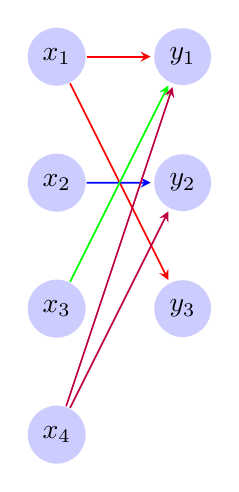
\begin{tikzpicture}[> = stealth, shorten > = 1pt, auto, node distance = 3cm, semithick, scale = .8, auto = left, every node/.style = {circle, fill=blue!20}]
    \node (x1) at (0, 0)   {$x_1$};
    \node (x2) at (0, -2)   {$x_2$};
    \node (x3) at (0, -4)   {$x_3$};
    \node (x4) at (0, -6)   {$x_4$};
    \node (y1) at (2, 0)   {$y_1$};
    \node (y2) at (2, -2)   {$y_2$};
    \node (y3) at (2, -4)   {$y_3$};
    \draw[red, ->] (x1) -- (y1);
    \draw[red, ->] (x1) -- (y3);
    \draw[blue, ->] (x2) -- (y2);
    \draw[green, ->] (x3) -- (y1);
    \draw[purple, ->] (x4) -- (y1);
    \draw[purple, ->] (x4) -- (y2);
    %\draw[red, ->, thick] (x1) arc (0:360:0.6);
\end{tikzpicture}
\end{center}

从上图我们可以得到:
\begin{enumerate}[a)]
    \item 关系图中表示最小元素的小圆圈,称为{\color{red}结点}(node);
    \item 表示元素间具有 $R$ 关系的{\color{red}有向线段}或{\color{red}有向弧},称为{\color{red}有向边}(directed edge);
    \item 起点和终点重合的有向边,成为{\color{red}环}(loop)或{\color{red}自回路};
    \item 关系 $R$ 的关系图记为 $G_R$。
\end{enumerate}
\subsection{关系的运算}
\begin{theorem}
    若 $Z$ 和 $S$ 是从 $X$ 到 $Y$ 的两个关系,则 $Z$,$S$ 的并、交、补、差仍是从 $X$ 到 $Y$ 的关系。
\end{theorem}
\begin{example}
    Let $R_1$ be the "less than" relation on the set of real numbers and let $R_2$ be the "greater than" relation on the set of real numbers, that is, $R_1 = \{(x, y) \mid x < y\}$ and $R_2 = \{(x, y) \mid x > y\}$. What are $R_1 \cap R_2$, $R_1 \cup R_2$, $R_1 - R_2$, $R_2 - R_1$, and $R_1 \bigoplus R_2$?
\end{example}
\begin{solve}
    We note that $(x, y) \in R_1 \cup R_2$ if and only if $(x, y) \in R_1$ or $(x, y) \in R_2$. Hence, $(x, y) \in R_1 \cup R_2$ if and only if $x < y$ or $x > y$. Because the condition
    $x < y$ or $x > y$ is the same as the condition $x \neq y$, it follows that $R_1 \cup R_2 = \{(x, y) \mid x \neq y\}$. In other words, the union of the "less than" relation and the "greater than" relation is the "not equal" relation.

    Next, note that it is impossible for a pair $(x, y)$ to belong to both $R_1$ and $R_2$ because it is impossible for $x < y$ and $x > y$. It follows that $R_1 \cap R_2 = \varnothing$.

    We also see that $R_1 - R_2 = R_1$, $R_2 - R_1 = R_2$, and $R_1 \bigoplus R_2 = R_1 \cup R_2 - R_1 \cap R_2 = \{(x, y) \mid x \neq y\}$.
\end{solve}
1. 逆关系:设 $R$ 为从 $A$ 到 $B$ 的二元关系,关系 $R$ 的逆($R$ 的{\color{red}逆关系})为 $R^{-1}$,定义为 $$R^{-1} = \{(b, a) \mid (a, b) \in R\}$$.

\begin{note}
    恒等关系的逆是恒等关系,空关系的逆是空关系,全域关系的逆是全域关系。
\end{note}
\begin{theorem}
    设 $R$,$R_1$,$R_2$ 是从 $A$ 到 $B$ 的二元关系,则
    \begin{enumerate}[a)]
        \item $(R^{-1})^{-1} = R$;
        \item $(R_1 \cup R_2) ^{-1} = R_1^{-1} \cup R_2^{-1}$;
        \item $(R_1 \cap R_2) ^{-1} = R_1^{-1} \cap R_2^{-1}$;
        \item $(R_1 - R_2)^{-1} = R_1^{-1} - R_2^{-1}$;
        \item $\overline{(R)}^{-1} = \overline{R^{-1}}$,(此处 $\overline{R} = A \times B - R$,称为 $R$ 的{\color{red}关系补})。
    \end{enumerate}
\end{theorem}
2. 复合关系:设 $R_1$ 为从 $A$ 到 $B$ 的关系,$R_2$ 为从 $B$ 到 $C$ 的关系,则 $R_1$ 和 $R_2$ 的{\color{red}复合关系}为从 $A$ 到 $C$ 的关系,记为 $R_1 \circ R_2$,定义为 $$R_1 \circ R_2 = \{(a, c) \mid a \in A \wedge c \in C \wedge (\exists b)(b \in B \wedge (a, b) \in R_1 \wedge (b, c) \in R_2)\}.$$ 其中 $\circ$ 表示{\color{red}关系的合成运算}。
\begin{note}
    关系的合成满足{\color{red}结合律}:$R_1 \circ (R_2 \circ R_3) = (R_1 \circ R_2) \circ R_3.$
\end{note}
3. 关系的幂:设 $R$ 是集合 $A$ 上的二元关系,$n \in \mathbb{N}$ 为任一自然数,则 $R$ 的 $n$ 次幂记为 $R^n$,定义为 $R^0 = \{(x, x) \mid x \in A\}$,$R^{n+1} = R^n \circ R$。
\begin{theorem}
    设 $R_1$ 为从 $A$ 到 $B$ 的关系,$R_2$ 为从 $B$ 到 $C$ 的关系,则 $$(R_1 \circ R_2)^{-1} = R_2^{-1} \circ R_1^{-1}$$
\end{theorem}
\begin{proof}
    $(c, a) \in (R_1 \circ R_2)^{-1} \\
    \Leftrightarrow (a, c) \in R_1 \circ R_2 \\
    \Leftrightarrow(\exists b)\left(b \in B \wedge\langle a, b\rangle \in R_{1} \wedge\langle b, c\rangle \in R_{2}\right) \\
    \Leftrightarrow(\exists b)\left(b \in B \wedge\langle b, a\rangle \in R_{1}^{-1} \wedge\langle c, b\rangle \in R_{2}^{-1}\right) \\
    \Leftrightarrow(c, a) \in R_{2}^{-1} \circ R_{1}^{-1}.$
\end{proof}
\subsubsection{关系的基本类型}
1. 自反性(reflexive):若对 $A$ 中的每一个 $x$,均有 $xRx$,则称 $R$ 是{\color{red}自反的},这对应着关系矩阵中主对角线元素全为 $1$,关系图中每个结点都有自环。

2. 对称性(symmetric):对每一个 $x, y \in A$,如果有 $xRy$ 都有 $yRx$,则称 $R$ 是{\color{red}对称的},这对应着关系矩阵为对称矩阵,关系图中的有向边成对出现。

3. 传递性(transitive):对于每一个 $x, y, z \in A$,如果有 $xRy, yRz$ 都有 $xRz$,则称 $R$ 是{\color{red}传递的},这对应着如果关系图中有一条从 $x$ 到 $z$ 的{\color{red}路径},则从 $x$ 到 $z$ 有一条弧。

4. 反自反性(irreflexive):若对 $A$ 中的每一个 $x$,均有 $x\cancel{R}x$,则称 $R$ 是{\color{red}反自反的},这对应着关系矩阵中主对角线元素全为 $0$,关系图中每个结点都没有自环。
\begin{note}
    “自反”的否定不是“反自反”,也就是说,一个不是自反的关系不一定就是反自反的。
\end{note}
5. 反对称性(antisymmetric):对每一个 $x, y \in A$,如果有 $xRy, yRx$,都有 $x = y$,则称 $R$ 是{\color{red}反对称的},这对应着如果关系图中有从 $a$ 到 $b$ 的弧,则必没有从 $b$ 到 $a$ 的弧。
\begin{note}
    与自反相同地,“对称”的否定不是“反对称”,一个关系可能既是对称的又是反对称的。不具备对称性的关系称为{\color{red}非对称关系}(asymmetric)。
\end{note}
\begin{theorem}
    若 $R$ 为 $A$ 上的关系,则
    \begin{enumerate}[a)]
        \item $R$ 在 $A$ 上自反,当且仅当 $I_A \subseteq R$.
        \item $R$ 在 $A$ 上反自反,当且仅当 $R \cap I_A = \varnothing$.
        \item $R$ 在 $A$ 上传递,当且仅当 $R \circ R \subseteq R$.
    \end{enumerate}
\end{theorem}
证明略去。
\begin{theorem}
    设 $R$ 为 $A$ 上的二元关系,则
    \begin{enumerate}[a)]
        \item $R$ 是对称的,当且仅当 $R^{-1} = R$.
        \item $R$ 是反对称的,当且仅当 $R \cap R^{-1} \subseteq I_A.$
    \end{enumerate}
\end{theorem}
同样略去证明。用关系矩阵可以直观的发现这一结论。

\subsection{关系的闭包}
1. 闭包:\textbf{包含}指定集合的满足某个运算下\textbf{闭合}的\textbf{最小集合}。

2. 设 $R$ 是 $A$ 上的二元关系,关系 $R'$ 是 $R$ 的{\color{red}自反闭包}(对称闭包、传递闭包),如果
\begin{enumerate}
    \item $R'$ 是\textbf{自反的}(对称的、传递的);
    \item $R \subseteq R'$;
    \item 对\textbf{任何自反的}(对称的、传递的)关系 $R''$,如果 $R \subseteq R''$,那么 $R' \subseteq R''$。
\end{enumerate}
$R$ 的自反、对称、传递闭包分别记作 $r(R),s(R),t(R)$。
\begin{theorem}
    设 $R$ 是集合 $A$ 上的关系,那么
    \begin{enumerate}
        \item $R$ 是自反的,当且仅当 $r(R) = R$;
        \item $R$ 是对称的,当且仅当 $s(R) = R$;
        \item $R$ 是传递的,当且仅当 $t(R) = R$。
    \end{enumerate}
\end{theorem}
3. 构造闭包的方法:设 $R$ 是集合 $A$ 上的二元关系,则
\begin{enumerate}
    \item 自反闭包 $r(R) = R \cup I_A$;
    \item 对称闭包 $s(R) = R \cup R^{-1}$;
    \item 传递闭包 $t(R) = \bigcup\limits_{i = 1}^{\infty} R^i = R \cup R^2 \cup \cdots$.
\end{enumerate}
\begin{proof}
    设 $R' = R \cup I_A$,下证 $R'$ 满足“自反闭包”的定义:
    \begin{enumerate}
        \item "$R'$ 是自反的":因为 $I_A \subseteq R'$;
        \item “$R \subseteq R'$”:由 $R' = R \cup I_A$;
        \item “对所有自反关系 $R''$,如果 $R \subseteq R''$,那么 $R' \subseteq R''$”:设 $R''$ 是自反的,则 $I_A \subseteq R''$。如果 $R \subseteq R''$,则 $$R' = R \cup I_A \subseteq R''.$$ 综上得证 $$r(R) = R \cup I_A.\ \QED$$
    \end{enumerate}
    设 $R' = R \cup R^{-1}$,下证 $R'$ 满足“对称闭包”的定义:
    \begin{enumerate}
        \item “$R'$ 是对称的”:$(x, y) \Longleftrightarrow (x, y) \in R \vee (x, y) \in R^{-1} \\
        \Longleftrightarrow (y, x) \in R^{-1} \vee (y, x) \in R \\
        \Longleftrightarrow (y, x) \in R'.$
        \item “$R \subseteq R'$”:由 $R' = R \cup R^{-1}$;
        \item “对任何对称关系 $R'‘$,如果 $R \subseteq R''$,那么 $R' \subseteq R''$”:下证任意 $(x, y) \in R'$,有 $(x, y) \in R''$:$$(x, y) \in R' \Longrightarrow (x, y) \in R \vee (x, y) \in R^{-1},$$
        \begin{enumerate}[(i)]
            \item $(x, y) \in R \Longrightarrow (x, y) \in R''$(由 $R \subseteq R''$);
            \item $(x, y) \in R^{-1} \Longrightarrow (y, x) \in R \subseteq R'' \Longrightarrow (x, y) \in R''$(由 $R''$ 是对称的)。
        \end{enumerate}
        综上得证 $$s(R) = R \cup R^{-1}.\ \QED$$
    \end{enumerate}
    对于 $t(R) = \bigcup\limits_{i = 1}^{\infty}R^i$,有 $$t(R) = \bigcup\limits_{i = 1}^{\infty}R^i {\color{red}\Longleftrightarrow} \left(\bigcup\limits_{i = 1}^{\infty}R^i \subseteq t(R)\right) \wedge \left(t(R) \subseteq \bigcup\limits_{i = 1}^{\infty}R^i\right).$$
    \begin{enumerate}
        \item 先证 $\bigcup\limits_{i = 1}^{\infty}R^i \subseteq t(R)$,用数学归纳法.
        \begin{enumerate}[a)]
            \item 由\emph{传递闭包}定义知,$R \subseteq t(R)$;
            \item 假定 $n \geq 1$ 时,$R^n \subseteq t(R)$,设 $(x, y) \in R^{n+1}$,则有 $$\begin{aligned}
                R^{n+1}=R^{n} \circ R & \Leftrightarrow(\exists c)\left(c \in A \wedge\langle x, c\rangle \in R^{n} \wedge\langle c, y\rangle \in R\right) \\
                & \Rightarrow(\exists c)(c \in A \wedge\langle x, c\rangle \in t(R) \wedge\langle c, y\rangle \in t(R)) \\
                & \Rightarrow\langle x, y\rangle \in t(R) \\
                & \Rightarrow R^{n+1} \subseteq t(R)
                \end{aligned}$$
        \end{enumerate}
        于是 $\bigcup\limits_{i = 1}^{\infty}R^i \subseteq t(R)$。
        \item 再证 $t(R) \subseteq \bigcup\limits_{i = 1}^{\infty}R^i$。由传递闭包 $t(R)$ 是包含 $R$ 的最小传递关系,往下只需要证明 $\bigcup\limits_{i = 1}^{\infty}R^i$ 是传递的。$$\begin{aligned}
            &\langle x, y\rangle \in \bigcup_{i=1}^{\infty} R^{i} \wedge\langle y, z\rangle \in \bigcup_{i=1}^{\infty} R^{i} \\
            \Leftrightarrow &(\exists s)(\exists t)\left(s \in \mathbb{N} \wedge t \in \mathbb{N} \wedge\langle x, y\rangle \in R^{s} \wedge\langle y, z\rangle \in R^{t}\right) \\
            \Leftrightarrow &\langle x, z\rangle \in R^{s} \circ R^{t}=R^{s+t} \\
            \Rightarrow &\langle x, z\rangle \in \bigcup_{i=1}^{\infty} R^{i} .
            \end{aligned}$$
        于是 $\bigcup\limits_{i = 1}^{\infty}R^i$ 是传递的。由于包含 $R$ 的传递关系都包含 $t(R)$,故 $t(R) \subseteq \bigcup\limits_{i = 1}^{\infty}R^i$。
        综上得证 $$t(R) = \bigcup\limits_{i = 1}^{\infty}R^i.\ \QED$$
    \end{enumerate}
\end{proof}
\begin{example}
    设 $A = \{a, b, c\}$,$R$ 是 $A$ 上的二元关系且 $R = \{(a, b), (b, c), (c, a)\}$,求 $t(R)$。
\end{example}
\begin{solve}
    对于关系 $R$,有 $$M_{R}=\left(\begin{array}{lll}
        0 & 1 & 0 \\
        0 & 0 & 1 \\
        1 & 0 & 0
        \end{array}\right)$$
        $M_{R^{2}}=\left(\begin{array}{lll}
            0 & 1 & 0 \\
            0 & 0 & 1 \\
            1 & 0 & 0
            \end{array}\right) \circ\left(\begin{array}{lll}
            0 & 1 & 0 \\
            0 & 0 & 1 \\
            1 & 0 & 0
            \end{array}\right)=\left(\begin{array}{lll}
            0 & 0 & 1 \\
            1 & 0 & 0 \\
            0 & 1 & 0
            \end{array}\right)$,\\
        $M_{R^{3}}=\left(\begin{array}{lll}
            0 & 0 & 1 \\
            1 & 0 & 0 \\
            0 & 1 & 0
            \end{array}\right) \circ\left(\begin{array}{lll}
            0 & 1 & 0 \\
            0 & 0 & 1 \\
            1 & 0 & 0
            \end{array}\right)=\left(\begin{array}{lll}
            1 & 0 & 0 \\
            0 & 1 & 0 \\
            0 & 0 & 1
            \end{array}\right)$,\\
        $M_{R^{4}}=\left(\begin{array}{lll}
            1 & 0 & 0 \\
            0 & 1 & 0 \\
            0 & 0 & 1
            \end{array}\right) \circ\left(\begin{array}{lll}
            0 & 1 & 0 \\
            0 & 0 & 1 \\
            1 & 0 & 0
            \end{array}\right)=\left(\begin{array}{lll}
            0 & 1 & 0 \\
            0 & 0 & 1 \\
            1 & 0 & 0
            \end{array}\right)$,

    注意到 $M_{R^4} = M_R$,于是 $R = R^4$。

    则有 $R = R^{3n+1},R^2 = R^{3n+2}, R^3 = R^{3n},(n = 1, 2, 3, \dots)$,故 $$\begin{aligned}
        t(R) &=\bigcup_{i=1}^{\infty} R^{i}=R \cup R^{2} \cup R^{3} \cup \cdots=R \cup R^{2} \cup R^{3} \\
        &=\{\langle a, a\rangle,\langle b, b\rangle,\langle c, c\rangle,\langle a, b\rangle,\langle b, c\rangle,\langle c, a\rangle,\langle b, a\rangle,\langle c, b\rangle,\langle a, c\rangle\}
        \end{aligned}.$$
\end{solve}
\begin{theorem}
    设 $R$ 是有限集合 $X$ 上的二元函数,$\mathrm{card}(X) = n$,则存在正整数 $k \leq n$,使得 $$t(R) = \bigcup\limits_{i = 1}^k R^i.$$
\end{theorem}
证明略去。由本定理可以得到,求传递闭包时上界可以写为 $n$ 而不必再写为 $\infty$。

4. Warshell 算法求传递闭包:
\begin{minted}{cpp}
    for(int k = 1;k <= n;k++)
        for(int i = 1;i <= n;i++)
            for(int j = 1;j <= n;j++)
                M[i][j] |= (M[i][k] & M[k][j]);
\end{minted}
时间复杂度为 $\mathcal{O}(n^3)$。
\begin{theorem}
    设 $R$ 是 $X$ 上的二元关系,则
    \begin{enumerate}
        \item $rs(R) = sr(R)$;
        \item $rt(R) = tr(R)$;
        \item $st(R) \subseteq ts(R)$.
    \end{enumerate}
    设 $R_1, R_2$ 为非空集合 $A$ 上的关系,且 $R_2 \subseteq R_1$,则
    \begin{enumerate}
        \item $r(R_2) \subseteq r(R_1)$;
        \item $s(R_2) \subseteq r(R_1)$;
        \item $t(R_2) \subseteq t(R_1)$。
    \end{enumerate}
\end{theorem}
证明略去。
5. 闭包在并运算上的分配律:
\begin{theorem}
    设 $R_1, R_2 \subseteq A \times A$ 且 $A \neq \varnothing$,则
    \begin{enumerate}
        \item $r(R_1 \cup R_2) = r(R_1) \cup r(R_2)$;
        \item $s(R_1 \cup R_2) = s(R_1) \cup s(R_2)$;
        \item $t(R_1 \cup R_2) \supseteq t(R_1) \cup t(R_2)$.
    \end{enumerate}
\end{theorem}
证明显然。
\subsection{等价关系和等价类}
1. 等价关系:设 $R$ 是非空集合 $A$ 上的二元关系,如果 $R$ 是自反的、对称的、传递的,则称 $R$ 为 $A$ 上的{\color{red}等价关系}。

2. 等价类:设 $R$ 为非空集合 $A$ 上的二元关系,$\forall a \in A$,令 $$[a]_R = \{x \mid x \in A \wedge aRx\}.$$则称 $[a]_R$ 为 $a$ 关于 $R$ 的{\color{red}等价类},简称为 $a$ 的等价类,简记为 $[a]$。
\begin{example}
    设 $A = \{a, b, c\}$,求等价关系 $$R=\{\langle a, a\rangle,\langle b, b\rangle,\langle c, c\rangle,\langle b, c\rangle,\langle c, b\rangle\}$$所有的等价类。
\end{example}
\begin{solve}
    $[a] = \{a\}, [b] = [c] = \{b, c\}$。
\end{solve}
\begin{theorem}
    设 $R$ 为非空集合 $A$ 上的等价关系,$\forall a, b \in A$,$$aRb \Longleftrightarrow [a]_R = [b]_R.$$
\end{theorem}
\begin{proof}
    \begin{enumerate}
        \item 若 $aRb$,则任取 $c \in [a]_R$,$$c \in[a]_{R} \Rightarrow a R c \Rightarrow c R a \Rightarrow c R b \Rightarrow b R c \Rightarrow c \in[b]_{R},$$故 $$[a]_R \subseteq [b]_R.$$
        同理可证 $[b]_R \subseteq [a]_R$,故 $[a]_R = [b]_R$。
        \item 反之,若 $[a]_R = [b]_R$,则 $$a \in [a]_R \Longrightarrow a \in [b]_R \Longrightarrow bRa \Longrightarrow aRb.\ \QED$$
    \end{enumerate}
\end{proof}
3. 商集:设 $R$ 是非空集合 $A$ 上的等价关系,集合 $\{[a]_R \mid a \in A\}$ 称为 $A$ 关于 $R$ 的{\color{red}商集}(quotient set),记作 $A / R$。
\begin{theorem}
    集合 $A$ 的一个划分确定 $A$ 的元素间的一个等价关系。
\end{theorem}
证明显然,此处略去。
\begin{theorem}
    若 $S = \{A_1, A_2, \dots, A_n\}$ 是非空集合 $A$ 上的划分,那么等价关系 $R$ 可以是 $$R = \bigcup\limits_{i = 1}^n A_i \times A_i.$$
\end{theorem}
4. $x \equiv y(\mathrm{mod}\ n) \Longleftrightarrow n | (x - y) \Longleftrightarrow x - y = kn(k \in \mathbb{Z})$,同余关系是等价关系。

5. 第二类 Stirling 数:把 $n$ 个不同的球放到 $k$ 个相同盒子中,要求无空盒,不同的方法总数 $\stirling{n}{k}$ 称为第二类 Stirling 数,也即把 $n$ 元集划分成 $k$ 个非空子集的分法总数。

递推式为 $\stirling{n}{k} = k\stirling{n - 1}{k} + \stirling{n - 1}{k - 1}.$ 考虑第 $n$ 个元素,如果它单独一个子集则方案数为 $\stirling{n - 1}{k - 1}$;如果它加入某一个子集中则方案数为 $k\stirling{n - 1}{k}$。

6. 贝尔数(Bell number):$B_n$ 为 $n$ 元集的划分方法的数目,其满足递推公式 $B_n = \sum\limits_{k = 0}^n C_n^k B_k$,同时也是相应的第二类 Stirling 数之和:$B_n = \sum\limits_{k = 0}^n \stirling{n}{k}.$

\subsection{相容关系}
1. 定义:集合 $A$ 上的二元关系 $r$ 称为{\color{red}相容关系},如果 $r$ 是自反的和对称的。
\begin{note}
    相容关系也可以满足{\color{red}传递性},也就是说,等价关系也是相容关系。

    相容关系也被称作{\color{red}相似关系}(similar relation)。
\end{note}
2. 相容类:设 $r$ 是集合 $A$ 上的相容关系,$C$ 是 $A$ 的子集,如果对于 $C$ 中任意两个元素 $a_1, a_2$ 有 $a_1 r a_2$,则称 $C$ 是由相容关系 $r$ 产生的{\color{red}相容类}。
如果一个相容类中再加入{\color{red}任一新元素},就不再组成相容类,就把这个相容类称作{\color{red}最大相容类}。

\subsection{序关系}
1. 全序关系:如果一个关系满足{\color{red}自反性,反对称性,传递性,强连通性},则称为{\color{red}全序关系}。
\begin{note}
    强连通性指的是任给两个元素 $x_1$,$x_2$,至少有 $x_1 R x_2$ 或 $x_2 R x_1$ 任意一个成立。
\end{note}
2. 偏序关系:如果一个关系满足{\color{red}自反性,反对称性,传递性},则称为{\color{red}偏序关系},称 $(\text{关系}, \text{集合})$ 为{\color{red}偏序集},偏序关系用 $\preccurlyeq$ 表示。
\begin{note}
    偏序也叫{\color{red}半序},当 $R$ 是偏序时,$aRb$ 就记为 $a \preccurlyeq b$。
\end{note}
3. “盖住”(覆盖)关系:设 $(A, \preccurlyeq)$ 为偏序集,$\forall x, y \in A$,如果 $x \preccurlyeq y, x \neq y$,且不存在 $z \in A$ 使得 $x \preccurlyeq z \preccurlyeq y$,则称 $y$ {\color{red}覆盖(盖住)} $x$。记作 $$\mathtt{COV} A = \{(x, y) \mid x, y \in A;y \text{盖住} x\}.$$

4. Hasse 图的画法:设有偏序集 $(A, \preccurlyeq)$,$\forall x, y \in A(x \neq y)$,适当排列结点的顺序,使得:
\begin{enumerate}
    \item 若 $x \preccurlyeq y$,则将 $x$ 画在 $y$ 的下方;
    \item 如果 $y$ 盖住 $x$,则用一条直线连接 $x$ 和 $y$。
\end{enumerate}
对于集合 $A = \{1, 2, 4, 6\}$ 的整除关系,其 Hasse 图如下:

\begin{center}
    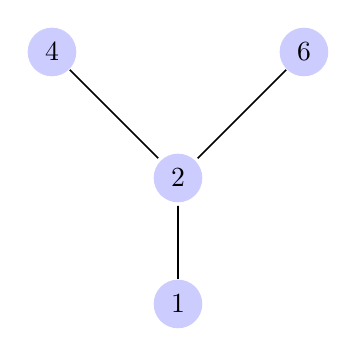
\begin{tikzpicture}[> = stealth, shorten > = 1pt, auto, node distance = 3cm, semithick, scale = .8, auto = left, every node/.style = {circle, fill=blue!20}]
    \node (x1) at (0, 0) {4};
    \node (x2) at (4, 0) {6};
    \node (x3) at (2, -2) {2};
    \node (x4) at (2, -4) {1};
    \draw (x1) -- (x3);
    \draw (x2) -- (x3);
    \draw (x4) -- (x3);
    %\draw[red, ->, thick] (x1) arc (0:360:0.6);
\end{tikzpicture}
\end{center}
\begin{note}
    Hasse 图中,无环,无有向边,无重边,无水平边,无由于传递性而形成的边。
\end{note}
5. 链:设 $(A, \preccurlyeq)$ 为偏序集,
\begin{enumerate}
    \item 在 $A$ 的一个子集中,如果每两个元素都是有关系的,则称这个子集为{\color{red}链}(chain);
    \item 在 $A$ 的一个子集中,如果每两个元素都是无关的,则称这个子集为{\color{red}反链}。
\end{enumerate}
\begin{note}
    通俗地讲,链中每两个元素都是可比的,反链中每两个元素都是不可比的。约定:如果一个集合是单元素集,那它既是链又是反链。
\end{note}
6. 全序关系:在偏序集 $(A, \preccurlyeq)$ 中,如果 $A$ 是一个链,则
\begin{enumerate}
    \item 称 $(A, \preccurlyeq)$ 为{\color{red}全序集合}(totally ordered set)或{\color{red}线序集合}(linearly ordered set);
    \item 二元关系 $\preccurlyeq$ 称为 $A$ 上的{\color{red}全序关系}(或{\color{red}线序关系})。
\end{enumerate}
7. 拓扑排序:
\end{document}

